\documentclass[conference]{IEEEtran}
\IEEEoverridecommandlockouts

\usepackage{cite}
\usepackage{booktabs}
\usepackage{multirow}
\usepackage{hyperref}
\usepackage{url}
\usepackage{subcaption}
\usepackage{float}
\usepackage{placeins}
\usepackage{svg}
\usepackage{amsmath,amssymb,amsfonts}
\usepackage{algorithmic}
\usepackage{graphicx}
\usepackage{textcomp}
\usepackage{xcolor}
\def\BibTeX{{\rm B\kern-.05em\textsc{i}\kern-.025em b\kern-.08em
    T\kern-.1667em\lower.7ex\hbox{E}\kern-.125emX}}
\begin{document}

\title{Comparing Convolutional and Recurrent Approaches for MEG Classification}

\author{\IEEEauthorblockN{Dani\"el Jochems}
\IEEEauthorblockN{David Huizinga}
\IEEEauthorblockN{Niek Grimbergen}
\IEEEauthorblockN{Daan van Dam}}

\maketitle

\begin{abstract}
Decoding brain activity with high accuracy is essential for advancing understanding of human cognition and 
neural processes. In this paper, we perform classification over magnetoencephalography (MEG) data to infer what
activity subjects are engaging in.  We experiment with both convolutional and recurrent neural network architectures, and
investigate whether attentional techniques can enhance performance. Furthermore, we examine how well these models generalize by comparing intra-subject and cross-subject classification scenarios. We found that the convolutional neural network outperformed
 the other models. Augmentation with attention techniques did not lead to better results, potentially indicating that a simpler model
 is better suited for learning on small datasets. all models exhibited a substantial drop in accuracy when applied to cross-subject classification, highlighting the challenge of inter-subject variability and domain shift in neural decoding tasks.




\end{abstract}

\section{Introduction}
Magnetoencephalography (MEG) is a non-invasive neuroimaging technique that measures the magnetic fields produced by electrical 
activity in the brain. Accurate classification of MEG data allows for use cases in brain-computer interfaces, medical diagnoses and
supports neuroscientific research \cite{belhadi2025eeg}. In this paper, we study whether it is possible to infer the cognitive task a subject is performing
based  on MEG recordings. To this end, we utilize deep learning techniques. Deep learning has proven effective in capturing complex, non-linear
 patterns in high-dimensional data \cite{lecun2015deep}, making it potentially well suited for the analysis of neuroimaging data. 

\section{Related Work}
While limited literature on MEG classification exists, EEG signal classification has been studied more intensively. Because of the
high degree of similarity between the two data sources, we expect previous research on EEG classification to be highly relevant.
Early work mainly utilized shallow methods like Support Vector Machines (SVMs) and other linear methods \cite{besserve2007classification}.
However, recent work \cite{lawhern2018eegnet} \cite{zhang2018cascade} \cite{abdellaoui2020deepbrainstateclassification}  has leveraged deep learning
techniques. EEGnet \cite{lawhern2018eegnet} is a compact Convolutional Neural Network (CNN) architecture  that has been designed for EEG signal classification. 
 Later, a combination of convolutional and recurrent techniques were utilized for the same task \cite{zhang2018cascade}. in \cite{abdellaoui2020deepbrainstateclassification} a similar approach is used,
but attention techniques popularized by transformer models \cite{vaswani2017attention} are adopted. 

\section{Methods}

\subsection{Model Selection}
To determine the best suited model architecture for the classification task, we considered both the nature of the data and the strength of various deep learning techniques.
 The selection of our model was guided by the two characteristics of the MEG data: the spatial structure of the various channels and the temporal dynamics.

\subsubsection{Spatial Considerations}
First of all, MEG data is created by recording the magnetic fields generated by electrical neural activity in the brain.
 This is achieved using a number of sensors attached to different parts of the scalp. Each individual sensor measures activity 
 in a specific area of the brain. This is the spatial structure. We want to select a model that can exploit this structure.
  Because of this, CNNs are well-suited, as these are specifically designed to capture spatial patterns.
CNNs can learn spatially localized patterns of activation that are characteristic of the different tasks to classify. 
CNN offers a degree of translation invariance, which means that it can produce the same output regardless of the input's position or location which should help with inter-subject variability. 

\subsubsection{Temporal Considerations}
Secondly, the data has a sequential nature: each training example consists of a sequence that develops over time, thus a time series. This introduces temporal dependencies that could be critical for accurate classification. Certain patterns may only be apparent through timing or duration. We need to choose a model that has the ability to capture these temporal dependencies. To this end, we can use Long Short-Term Memory networks (LSTMs). LSTMs are a type of Recurrent Neural Network designed to model long-range temporal dependencies and mitigate vanishing gradient problems. We could also choose a transformer model, which is able to outperform LSTM in a similar temporal dependent classification task \cite{ali2024comprehensive}, however, since we are dealing with a small dataset and transformers are data-intensive it would likely underperform due to insufficient training data. 

\subsubsection{Attention Mechanisms}
We also explore some models that use attention mechanism, which can dynamically weigh the importance of different time steps during classification. Attention provides the model the flexibility to focus on the most relevant segments of a MEG sequence for each prediction. This is in contrast to processing all time steps equally. This approach could be particularly beneficial for MEG data, where a task-relevant activity may occur at a specific latencies post-stimulus. We apply this on top of CNN or LSTM outputs to capture these time-varying relevances to complement.

In summary, we experiment using two different architectures: a CNN, which we selected to capture spatial structure, and an LSTM, which can model temporal dependencies. Additionally, we augment the CNN architecture with self attention, as well as multi-headed attention.

\section{Data Preprocessing}
\subsubsection{Normalization}
To normalize the data, we applied min-max scaling, bringing each feature to the $[0,1]$ range based on the global minimum and maximum values computed from the entire training set.
 This approach preserves the relative structure of the data while ensuring all features operate on a comparable scale, especially with sensor-based time-series inputs.
The normalization is implemented in the scale data function and applied uniformly to both training and test sets, using the training statistics only. We do this to ensure consistency across the entire pipeline.

\subsubsection{Downsampling}
We applied uniform downsampling to the data to reduce temporal resolution and computational load. 
This is done by selecting a fixed proportion of timesteps in evenly spaced intervals across the full sequence, in our case we chose this to be 20 percent. This value was chosen to have everything still fit within the memory of the PC we ran this on. Additionally, using all of the data might make the model prone to overfitting. With this implementation we compute the stride based on the downsampling factor and select indices accordingly, ensuring consistent coverage of the original signal. 

\subsection{Model Descriptions}
\begin{tabular}{ll}
    \toprule
    Model & Key layers (in order) \\
    \midrule
    \multirow{5}{*}{LSTM}            & Input $(7124{\times}248)$\\
                                     & LSTM 64\\
                                     & Dense 64 (ReLU)\\
                                     & Dropout 0.2\\
                                     & Dense 4 (softmax)\\
    \midrule
    \multirow{5}{*}{Bi-LSTM}         & Input $(7124{\times}248)$\\
                                     & Bi-LSTM 64\\
                                     & Dense 64 (ReLU)\\
                                     & Dropout 0.2\\
                                     & Dense 4 (softmax)\\
    \midrule
    \multirow{5}{*}{CNN}             & Conv1D 64, $k{=}5$\\
                                     & MaxPool 2\\
                                     & Conv1D 128, $k{=}5$\\
                                     & GlobalAvgPool\\
                                     & Dense 64$\rightarrow$4\\
    \midrule
    \multirow{5}{*}{CNN+Self-Attn}   & Conv1D 64, $k{=}5$\\
                                     & MaxPool 2\\
                                     & Conv1D 128, $k{=}5$\\
                                     & Self-Attention\\
                                     & Dense 64$\rightarrow$4\\
    \midrule
    \multirow{5}{*}{CNN+MH-Attn}     & Conv1D 64, $k{=}5$\\
                                     & MaxPool 2\\
                                     & Conv1D 128, $k{=}5$\\
                                     & Multi-Head (4$\times$32)\\
                                     & Dense 64$\rightarrow$4\\
    \bottomrule
    \end{tabular}

 \subsection{Hyperparameter Tuning}
 For both the CNN and LSTM models, we selected hyperparamters based partly on what is commonly used in related deep learning tasks, and partly on manual experimentation.
 
 The CNN was trained using the Adam optimizer with a learning rate of 0.001. This relatively low value helps to avoid unstable training and makes small, careful updates to the model weights, which is useful for deep architectures like CNNs that see more chaotic convergence than simpler models. The LSTM used the default learning rate of 0.001, since it has fewer parameters and seemed to benefit from slightly faster learning in early epochs. No full grid search was done, but different values were tested emperically to see what gave the most stable validation accuracy.
 
 During training, we used a batch size of 4. For validation and testing, this was set to 1 or 2. This was mostly done to ensure there were no out of memory errors during training.
 
 After the dense layers dropout layers were added to promote generalisation. In the CNN a dropout rate of 0.08 was used, compared to 0.2 in the LSTM. The LSTM needed a higher rate to regularize the temporal memory better. These values where based on a few experiments where higher dropout started to hurt the performance. 
 
 The CNN had two convolutional layers with 64 and 128 filters, followed by global average pooling and dense layers of size 16 and 64. The LSTM had a single LSTM layer with 64 units, which was followed by a 64 unit dense layer. These hyperparameters were selected to provide enough capaciy to model the data without making the networks too large to train.The number of layers were not searched extensively, but chose values based on prior knowledge and experimentation.
 
 As the number of epochs during training, early stopping was used with a maximum of 1000 epochs. This was done to prevent overfitting, and so that when the model is no longer improving on validation loss the training is stopped. A patience of 10 was used, meaning the model was allowed to train for up to 10 additional epochs without improvement before stopping. This number was chosen to give the model the chance to escape local minima, but avoid overfitting on the training data. The option to restore the best weights was added so that after stopping, the model automatically reverts to the state with the lowest recorded validation loss.
 
\section{Results}

\section{Intra results}
Regarding training on intra, all five models achieved a perfect accuracy score of 1.0000. This indicates that the models were able to accurately distinguish between task conditions when trained and tested on data from the same individual. Signal characteristics such as baseline levels, noise patterns, and spatial configurations were consistent, which allowed the models to learn subject-specific patterns effectively.

\begin{figure*}[t]
    \centering
    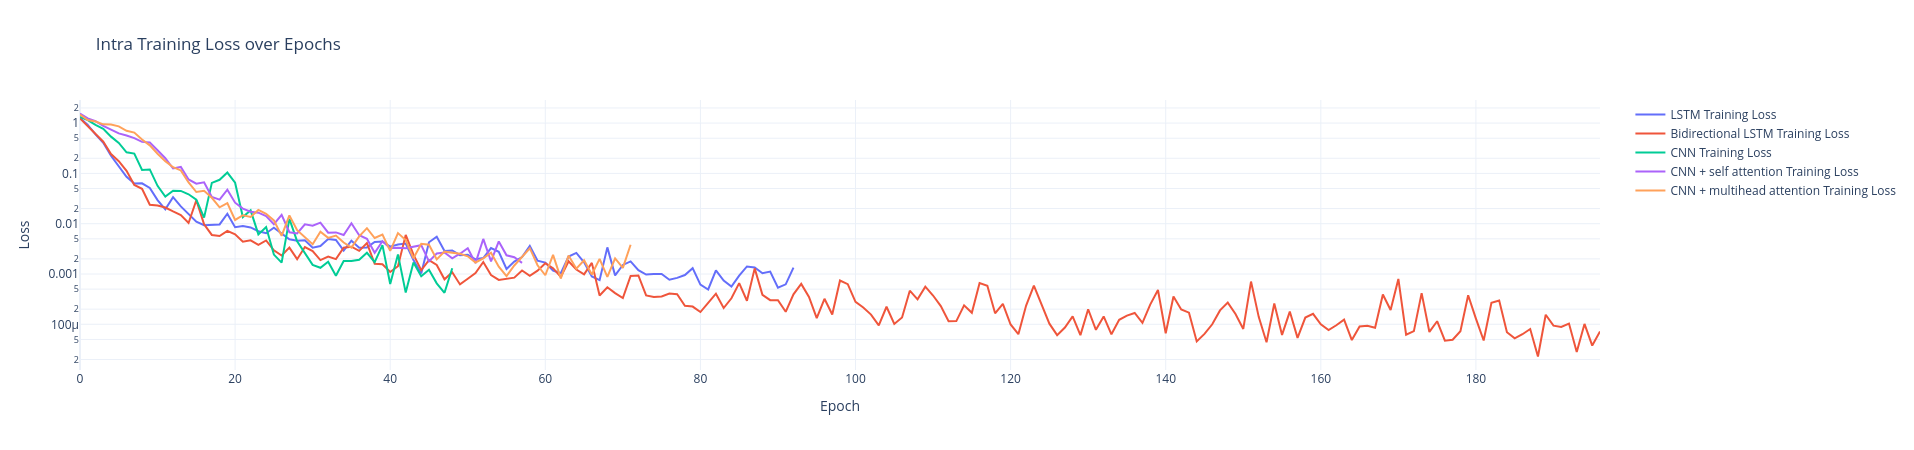
\includegraphics[width=\textwidth]{figures/loss_intra_res.png}
    \caption{Loss over epochs for the intra-subject classification models.}
    \label{fig:intra_loss_over_epoch}
\end{figure*}

In the loss values (Figure \ref{fig:intra_loss_over_epoch}) there are some differences between the models, which reflect the confidence with which predictions where made. The Bidirectional LSTM achieved the lowest loss (0.000012) at 187 epochs (excluding the patience of 10), followed by the standard LSTM (0.000349) at 83 epochs, indicating strong performance by both recurrent architectures. Among the convolutional models, the CNN with multihead attention produced the lowest loss (0.000837) at 62 epochs, slightly outperforming the plain CNN (0.001463) at 39 epochs and the CNN with self-attention (0.001732) at 48 epochs. These results confirm that intra-subject classification is a relatively easy task for deep learning models, but differences in loss values can be achieved by using different kinds of models.

\subsection{Cross results}
For the cross results multiple models were trained on the same underlying training set using the same preprocessing. The results for the training loss over the epochs is shown in Figure \ref{fig:cross_loss_over_epoch}. The LSTM models here clearly stop much earlier than the CNN models. In particular the \textsc{lstm-model} stops very early, at around $30$ epochs, the loss gradually lowers, but as soon as it starts overgeneralising and no improvement is made the early stopping causes it to stop. This happens later with the \textsc{bidirectional-lstm-model} because it not only looks back at the past but also at the future, which allows it to learn more complex patterns. The \textsc{cnn-model} does not take this temporal aspect into account and simply learns a complex representation of the training data over the entire set. The loss curve gradually goes down, but it is choppy because of the stochastic optimisation method we utilize. This method allows some temporary loss increases to ensure local minima are avoided.  The \textsc{cnn-self-attention-model} and \textsc{cnn-multi-head-model} both have a similar loss curve, but the \textsc{cnn-multi-head-model} captures more features at once, where each head focuses on different parts of the input, but requiring more elaborate learning because of its increased parameter count.

\begin{figure*}[t]
    \centering
    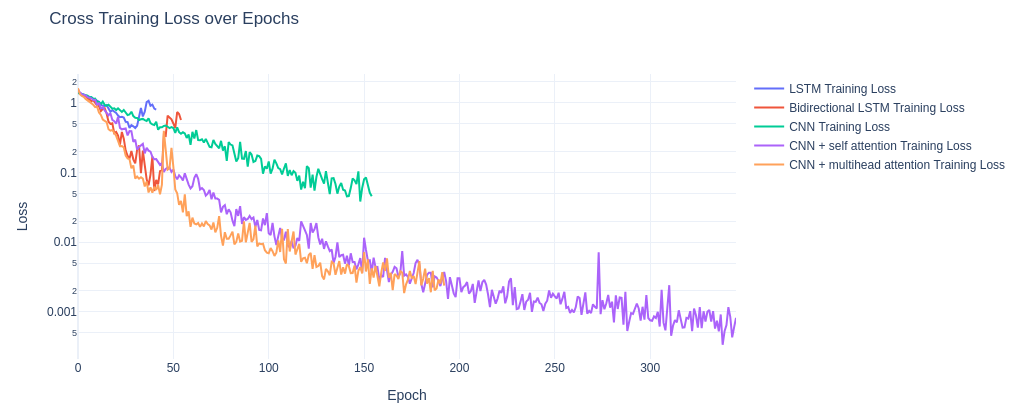
\includegraphics[width=\textwidth]{figures/cross_loss_over_epoch_small.png}
    \caption{Loss over epochs for the cross-subject classification models.}
    \label{fig:cross_loss_over_epoch}
\end{figure*}

The results for training accuracy are shown in Figure \ref{fig:cross_accuracy_over_epoch}. The x-axis here is the same and we generally see that it settles on accuracies much quicker then it decreases the loss. This makes sense because the loss function captures more subtle improvements. The accuracies in comparison are more rigid. The predicted class is either wrong or correct. Once the model gets the predictions correct it will not improve. Each of the models is a good fit for the training data just like the intra classifier.

\begin{figure*}[t]
    \centering
    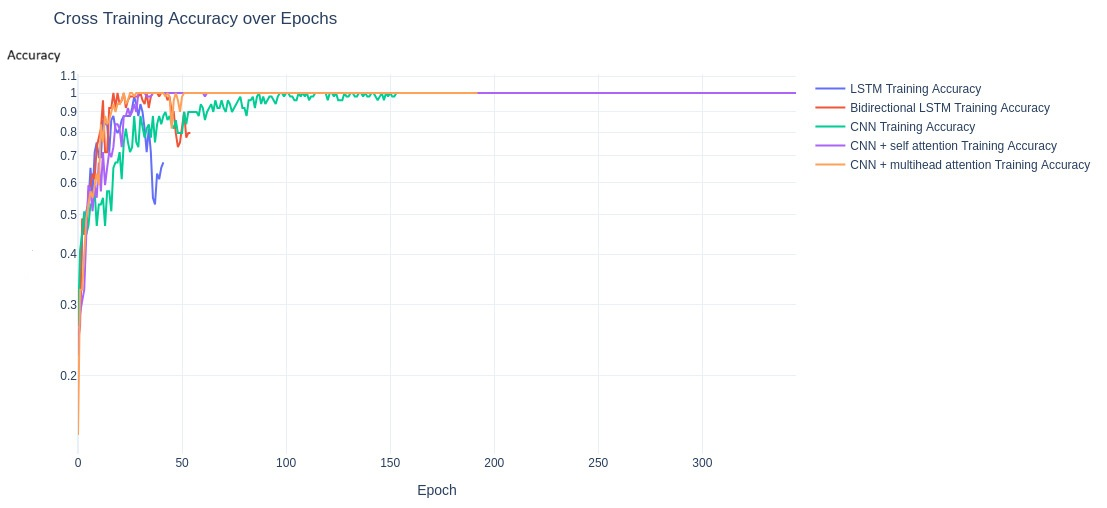
\includegraphics[width=\textwidth]{figures/accuracy graph_over_epochs_small_new.jpg}
    \caption{Accuracy over epochs for the cross-subject classification models.}
    \label{fig:cross_accuracy_over_epoch}
\end{figure*}

The test losses are showcased in Figure \ref{fig:test_loss_bars}. It is obvious here that the loss levels on the test sets can differ significantly versus the training. Generally the losses in the CNN models for both test set 1 and 2 are either equal or lower to that of the LSTM models. Looking at the \textsc{CNN-attention-model} and \textsc{cnn-multi-head-model}, test set 3 is either equal or lower to the \textsc{LSTM-model}, whereas the for test set 1 the loss is quite a bit lower in all CNN models. However test set 2, which we establish later is very different from the training set, this can have several possible explanations. Because the LSTM has a lower loss it could be that test set 2 contains data characterstics that CNNs struggle with such as long-range or sequential dependencies. More in depth reasoning as to why test set 2 shows anomalous behaviour is discussed later. All the results for the cross-subject classification models are shown in Table \ref{tab:cross_model_results}.

\begin{figure*}[t]
    \centering
    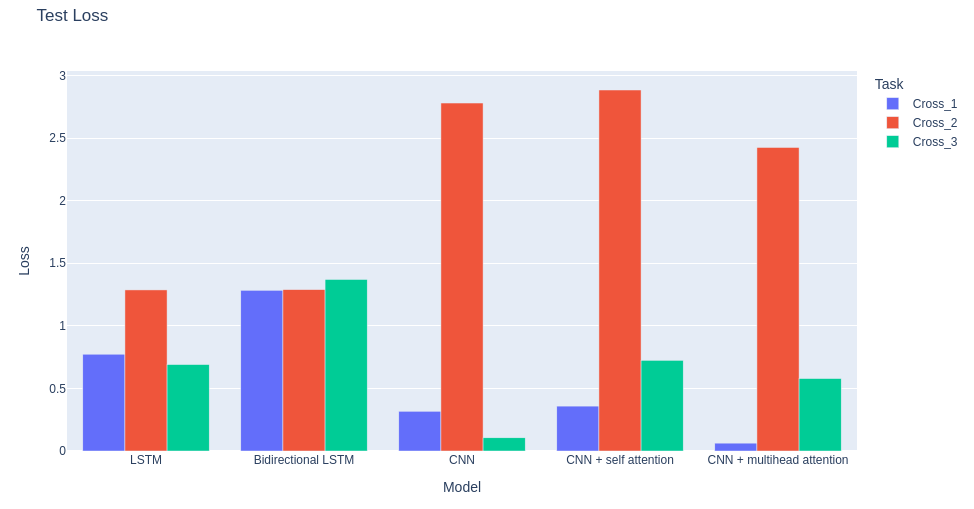
\includegraphics[width=\textwidth]{figures/test_loss_bars.png}
    \caption{Test loss for the cross-subject classification models. The x-axis shows the model, and the y-axis shows the loss. The bars are grouped by test set.}
    \label{fig:test_loss_bars}
\end{figure*}



\begin{table}[H]
    \centering
    \caption{Loss and Accuracy per Model and Task}
    \begin{tabular}{|c|l|l|c|c|}
    \hline
    \textbf{Model} & \textbf{Task} & \textbf{Loss} & \textbf{Accuracy} \\
    \hline
    LSTM                    & Cross\_1                  & 0.773341  & 0.6875 \\
    LSTM                    & Cross\_2                  & 1.286765  & 0.4375 \\
    LSTM                    & Cross\_3                  & 0.690458  & 0.7500 \\
    Bidirectional LSTM     & Cross\_1                  & 1.283687  & 0.6875 \\
    Bidirectional LSTM     & Cross\_2                  & 1.289164  & 0.3750 \\
    Bidirectional LSTM     & Cross\_3                  & 1.370187  & 0.5000 \\
    CNN                    & Cross\_1                  & 0.317381  & 0.8750 \\
    CNN                    & Cross\_2                  & 2.779860  & 0.5000 \\
    CNN                    & Cross\_3                  & 0.105421  & 1.0000 \\
    CNN + self attention   & Cross\_1                  & 0.358578  & 0.8750 \\
    CNN + self attention   & Cross\_2                  & 2.883909  & 0.4375 \\
    CNN + self attention   & Cross\_3                  & 0.724158  & 0.6875 \\
    CNN + multihead attention & Cross\_1              & 0.062801  & 1.0000 \\
    CNN + multihead attention & Cross\_2              & 2.424778  & 0.5000 \\
    CNN + multihead attention & Cross\_3              & 0.578709  & 0.7500 \\
    \hline
    \end{tabular}
    \label{tab:cross_model_results}
    \end{table}
    

\section{Discussion}

\subsection{Accuracy differences Intra vs Cross}
In intra-subject classification, both training and testing data come from the same subject. This means that signal characteristics (sensor placements, movements, physiology) are consistent between readings. The distribution of the test data is also very similar to the training data. This allows for really fine-grained patterns specific to the person, explaining the high accuracy. 

Cross-subject classification, however, performs worse due to the signal characteristics being variable. The trouble then comes from overfitting to the train subjects, which may or may not share physiological and behavioural similarities, and/or sensor placements with the test subjects. The model then learns patterns not represented in some testing cases. One could generalise, which can increase accuracy for lacking test sets, but lowers the score of test sets that were highly similar to the training set. Clearly from testing both test set 1 and 3 fall within the feature distribution, whereas test set 2 does not. This can be beacuse of again physiological differences, but could also be because it is noisy or low-quality data, a different baseline or signal range. This is commonly reffered to as a domain shift.

To improve cross-subject generalisation one could normalise data per subject to reduce individual differences, use transfer learning or domain-invariant representations, use meta learning to train models that can then quickly adapt to a new subject it sees during training, feature engineering to construct features that are invariant across people, or of course more data.

For example, we normalise based only on the training set. If test set 2 contains a different baseline then scaling test set 2 using those values from an unrelated distribution may distort the data. Performing t-SNE separately on the training and test sets to show label-wise distribution (task states) shows that the classes are fairly-well separated. This suggests that a classifier should be able to separate these labels provided the test data lies in the same distribution. However, showing source-wise distribution we can tell that test set 1 and 3 overlap significantly with the train distribution (Figure \ref{fig:tsne_distribution_shift}). Test 2 however is slightly shifted. Computing the centroid distance in t-SNE space between each test set and the train set shows that test 2 is clearly most shifted. This aligns with classifier results.

\label{discussion}
An attempt was made to do some specific MEG preprocessing like namely, a fixed bandpass filter, prepare channel z-scoring, and baseline correction. The inspiration for these came from the \href{https://mne.tools/stable/index.html}{MNE tools} package and the corresponding paper by Gramfort et al \cite{gramfort2013meg}. This applied preprocessing before model training severaly impacted results.Together they destroyed the signal for effective classification, rendering the model useless at classifying. Per channel z-scoring alone was effective however. 

Some experimentation was done to leave a smaller memory footprint when training for the cross-subject classification model because of the size of the matrices. The approach was to extract features from the training data so there was no need for excessively downsampling on the time points. This was done by capturing signal amplitude statistics from the data which are the mean signal per channel, signal variability, peak and minimum amplitude, and the dynamic range of the channels. Some domain knowledge and assumptions are made here where high-amplitudes signify movement tasks, whereas low-amplitudes signify rest signals. Subsequently a discrete fourier transformation was done over the channels, to determine average frequency content and variability in frequencies. The reason is to capture distinct frequency signatures of the different tasks. Lastly cross-channel correlation was performed and only the upper triangle of the correlation matrix was kept, to not involve redundant information. These 'features' were flattened into a single vector for use in training. This creates a high-dimensional vector per sample. These features for the training data and the test data were scaled using the 'StandardScaler' from sklearn. Afterwards PCA was performed to reduce the dimensions of the data and keep $95\%$ of the variance and these were used in training the model. This was ultimately fed into a simple feedforward model (\textsc{pca-feedforward-model}) The accuracy for getting the correct task in the test sets $1$, $2$, and $3$ were $0.88$, $0.25$, and $0.70$ respectively. To explain this phenomenon t-SNE was performed on the training and test data to assess distribution overlap of Train vs Test1/2/3 (Figure \ref{fig:tsne_distribution_shift}). While Test 1 and 3 overlap significantly with the train distribution, test 2 is shifted signifying a distribution shift. This cannot be because of a class imbalance, because the task label distributions are equal. Similarly the centroid distance in t-SNE space between each test set and the Train set was computed (Table \ref{tab:centroid_distance}). Where it is clear again that test set 2 is shifted compared to the training set. This all indicates a domain shift. One could leverage a domain adaptation model, augment the train data to generalise better, or use a different model that is more robust to distribution shifts.

This \textsc{pca-feedforward-model} has a benefit that it is a simple model that trains very quickly ($100$ milliseconds per epoch) because of the feauture engineering step beforehand. Training a model of moderate accuracy for test set 1 and 3 is done under a minute on a single thread. This is an advantage when comparing to the other proposed models which take many minutes to hours. But the results are not very good for test set 2. This is likely because the model is not robust to distribution shifts because of its simplicity.

\section{Limitations}
Several constraints influenced the design choices and model performance. Firstly, hyperparameters such as learning rate, dropout, and model size were first tuned experimentally through minimal experimentation rather than systematic search. This was due to a computational constraint, where available memory constrained the ability to conduct extensive grid searches or parallel experiments.

Second, the data was also considerably downsampled to reduce the temporal resolution and make training computationally feasible. While this minimized the memory requirement, this removed potentially informative temporal detail from the MEG signals, which might have had a negative impact on the model's ability to detect fine-grained patterns.

Finally, the overall number of training samples was limited. Especially in the cross-subject scenario, the available data per subject and per class constrained the models' capabilities to generalize beyond the training distribution. It made it more difficult to assess the full potential of the selected architectures under more data-abundant conditions.

\section{Conclusion}
In this study, we explored the application of deep learning models to MEG data classification, comparing both intra-subject and cross-subject performance across multiple architectures. These architectures include CNNs, LSTMs, and attention-augmented CNNs. Our findings demonstrate that intra-subject classification provides significantly higher accuracy, with CNNs outperforming other architectures in this setting. However, we observed a notable drop in performance when applying models to cross-subject classification. We expect this occurs because of domain shift issues. These results emphasize the necessity for more robust methods to handle inter-subject variability in MEG data. Future work could explore domain adaptation techniques, contrastive learning, or alignment strategies to mitigate these effects. Ultimately, improving cross-subject generalization is critical for translating MEG-based brain decoding models to real-world applications such as brain-computer interfaces and clinical diagnostics.



\section*{AI Statement}
We consulted ChatGPT for our model choice, suggestions on normalization and downsampling techniques, and general questions during debugging.  We used it to transform panda dataframes
into graphs. It was used to spell check and detect general errors in the writing.
\bibliographystyle{IEEEtran}
\bibliography{references}

\clearpage
\onecolumn

\section*{Supplementary Materials}
\begin{figure}[H]
    \centering
    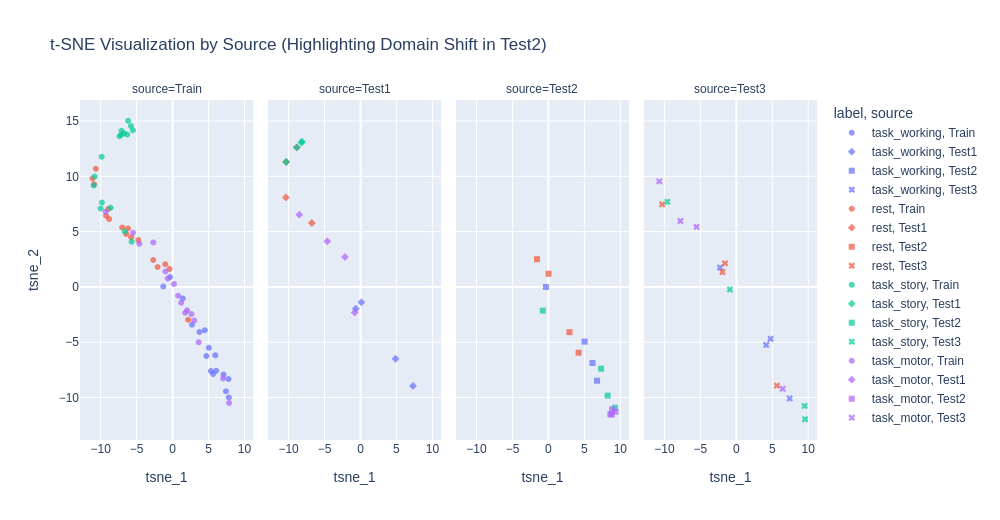
\includegraphics[scale=.5]{figures/supplementary_distribution shift test set 2.png}
    \caption{Here the t-SNE  embedding dimensions of the training set and test sets. This is the dimension reduction done on the distribution of the principal components of the original data. It shows the clustering of those points in the t-SNE space. Here we can see that test set 1 resembles the training set the most, after this test set 3, and finally test set 2 which is clearly shifted. This is in accordance with \textsc{pca-feedforward-model}}
    \label{fig:tsne_distribution_shift}
\end{figure}

\begin{table}[H]
    \centering
    \begin{tabular}{|c|c|c|}
        \hline
        Test Set & Centroid Distance to Train (t-SNE) & Avg Distance to Train Samples \\
        \hline
        \textbf{Test 2} & \textbf{37.62} & \textbf{47.49} \\
        Test 3 & 15.02 & 26.80 \\
        Test 1 & 12.82 & 23.91 \\
        \hline
    \end{tabular}
    \caption{Centroid distance between train and test sets in t-SNE space. Showcasing the distribution shift of test set 2 compared to the training set. Test set 2 is clearly the most shifted because its centroid is further away from the train centroid. On average every test set 2 sample is more distant from the train samples.}
    \label{tab:centroid_distance}
\end{table}

\subsection{Github Repository Link}
\url{https://github.com/DanielvanDamme/DL25-Groep-DDDN/tree/main/assignment%201/code}
\end{document}
